\documentclass[10pt,a4paper]{article}
\usepackage[latin1]{inputenc}
\usepackage[english]{babel}
\usepackage{amsmath}
\usepackage{amsfonts}
\usepackage{amssymb}
\usepackage{graphicx}
\usepackage{fancyhdr}
\usepackage{lastpage}
\usepackage{multirow}

%Include and define  c code
\usepackage{listings}
\usepackage{color}
\usepackage{textcomp}
\definecolor{listinggray}{gray}{0.9}
\definecolor{lbcolor}{rgb}{0.9,0.9,0.9}
\lstset{
	language=C,
	keywordstyle=\bfseries\ttfamily\color[rgb]{0,0,1},
	identifierstyle=\ttfamily,
	commentstyle=\color[rgb]{0.133,0.545,0.133},
	stringstyle=\ttfamily\color[rgb]{0.627,0.126,0.941},
	showstringspaces=false,
	basicstyle=\small,
	numberstyle=\footnotesize,
	numbers=left,
	stepnumber=1,
	numbersep=10pt,
	tabsize=2,
	breaklines=true,
	prebreak = \raisebox{0ex}[0ex][0ex]{\ensuremath{\hookleftarrow}},
	breakatwhitespace=false,
	aboveskip={1.5\baselineskip},
  columns=fixed,
  upquote=true,
  extendedchars=true,
 frame=single,
 backgroundcolor=\color{lbcolor},
}

\oddsidemargin  -0.5cm
\evensidemargin 0.0cm
\textwidth      17.25cm
\headheight     1.0cm
\headsep		0.7cm
\topmargin      -0.5cm
\textheight		22.0cm

\pagestyle{fancy}
\lhead{Exercise 5}
\chead{EEMB1}
\rhead{\thepage\ of \pageref{LastPage}}
\lfoot{Theis Christensen\\Paulo Fontes\\Dennis Madsen}
\cfoot{Team3}
\rfoot{\today}
\renewcommand{\headrulewidth}{0.4pt}
\renewcommand{\footrulewidth}{0.4pt}
\begin{document}
\part*{EEMB1 - KK - Assignment 6}
\section{Introduction}
The goal of this exercise was to create a circular buffer, containing the functions: \textit{put, get, isEmpty, isFull, initialise.}
The buffer should be able to either overwrite if the buffer is full or return false (specified under initialization). The program
must not contain any form of console interaction.
A good thing could be to try designing the program using the programmers main design tool (pen and paper), but mostly I just used the:
\\ \newline
\begin{figure}[h!]		%Remember to put the h!, to not fuck the sections.
	\begin{centering}
 		
\includegraphics[width=0.6\textwidth]{brain.jpg}
		\caption{A brain}
	\end{centering}
\end{figure}

\newpage
\section{Sketching}
\subsection{Test}
Well, some of the things has also been written down.
The first 3 pictures are the ideas about what elements the test function should contain.
\begin{figure}[th!]		%Remember to put the h!, to not fuck the sections.
 	\begin{centering}
 		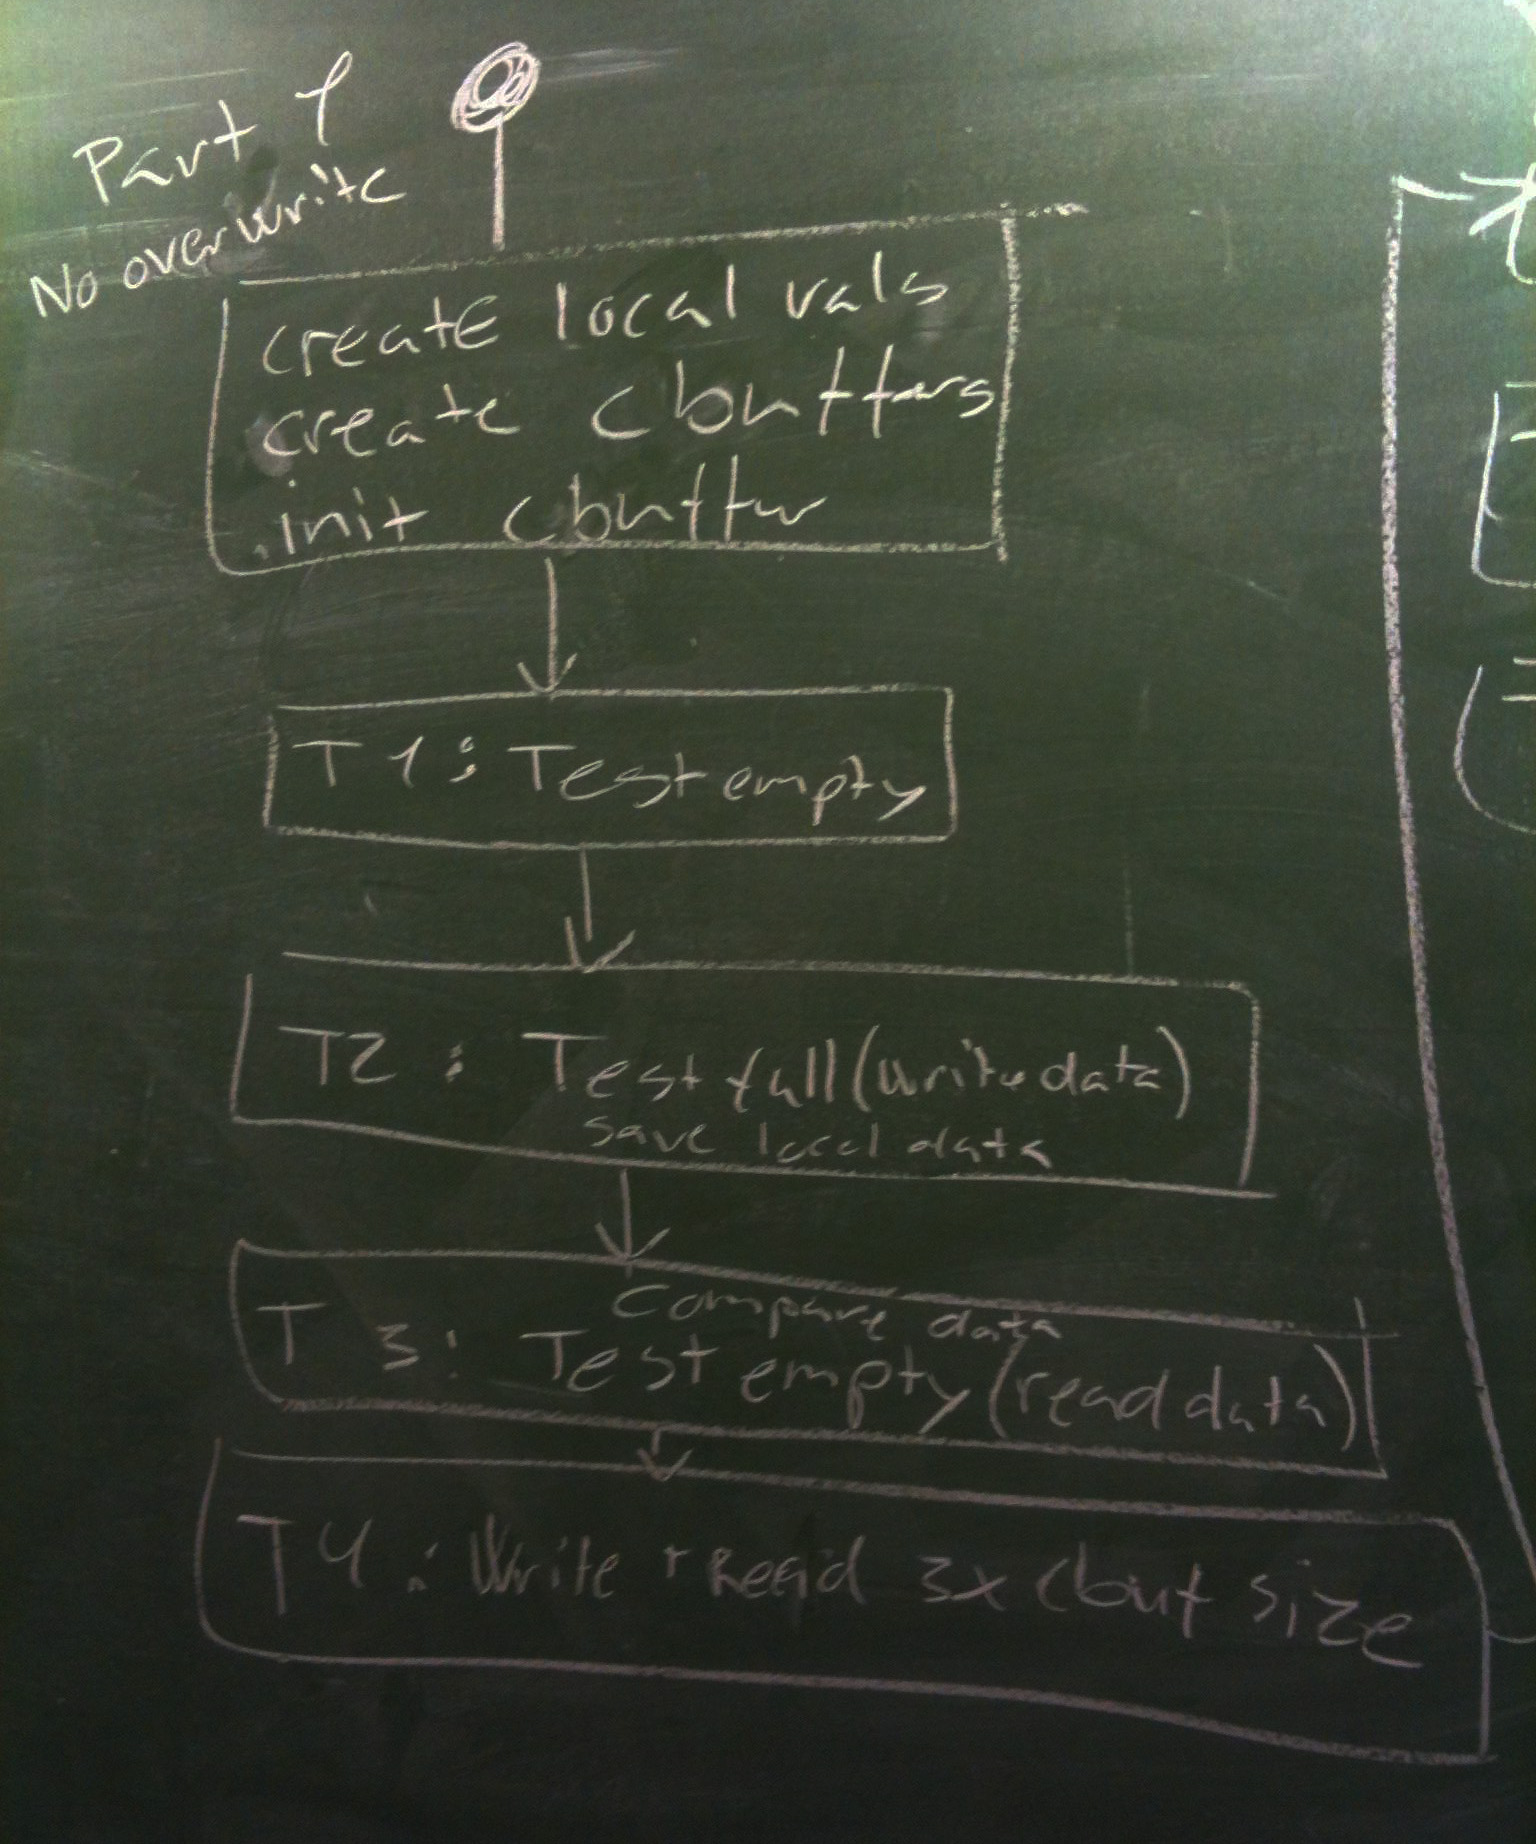
\includegraphics[width=0.7\textwidth]{part1.jpg}
		\caption{Part one of the test, NO overrun mode}
	\end{centering}
\end{figure}
\newpage
\begin{figure}[th!]		%Remember to put the h!, to not fuck the sections.
	\begin{centering}
 		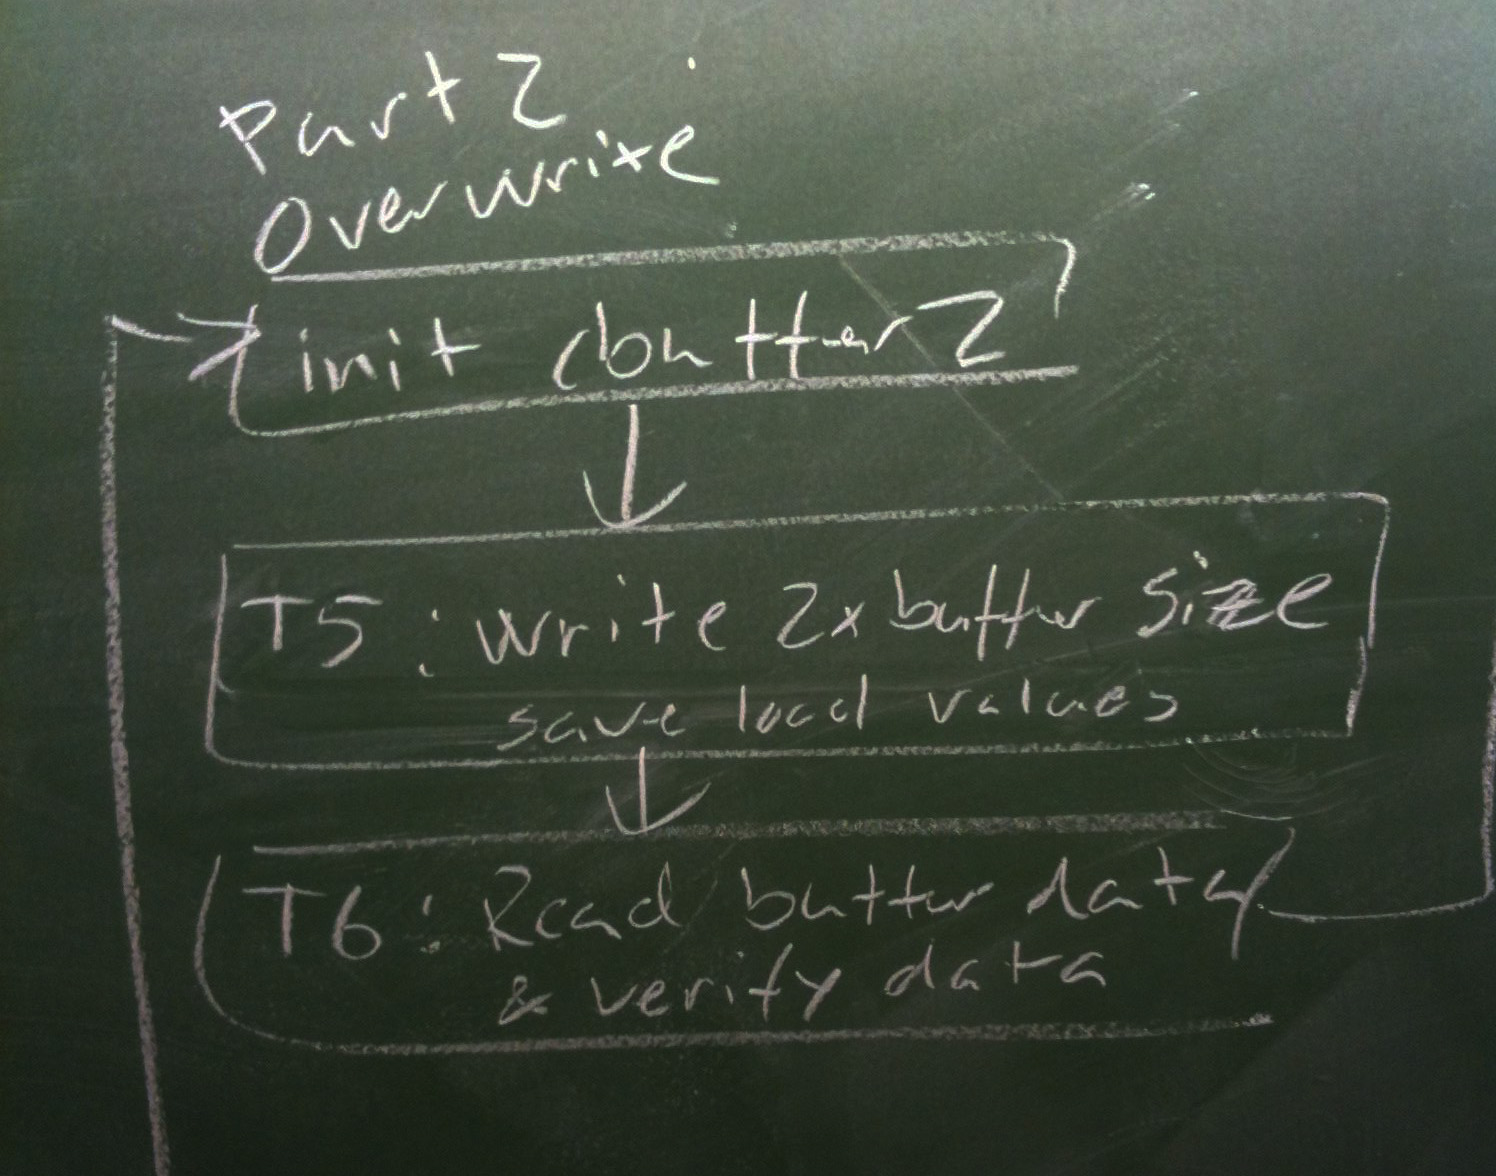
\includegraphics[width=0.6\textwidth]{part2.jpg}
		\caption{Part two of the test, Overrun mode ON}
	\end{centering}
\end{figure}

\begin{figure}[bh!]		%Remember to put the h!, to not fuck the sections.
	\begin{centering}
 		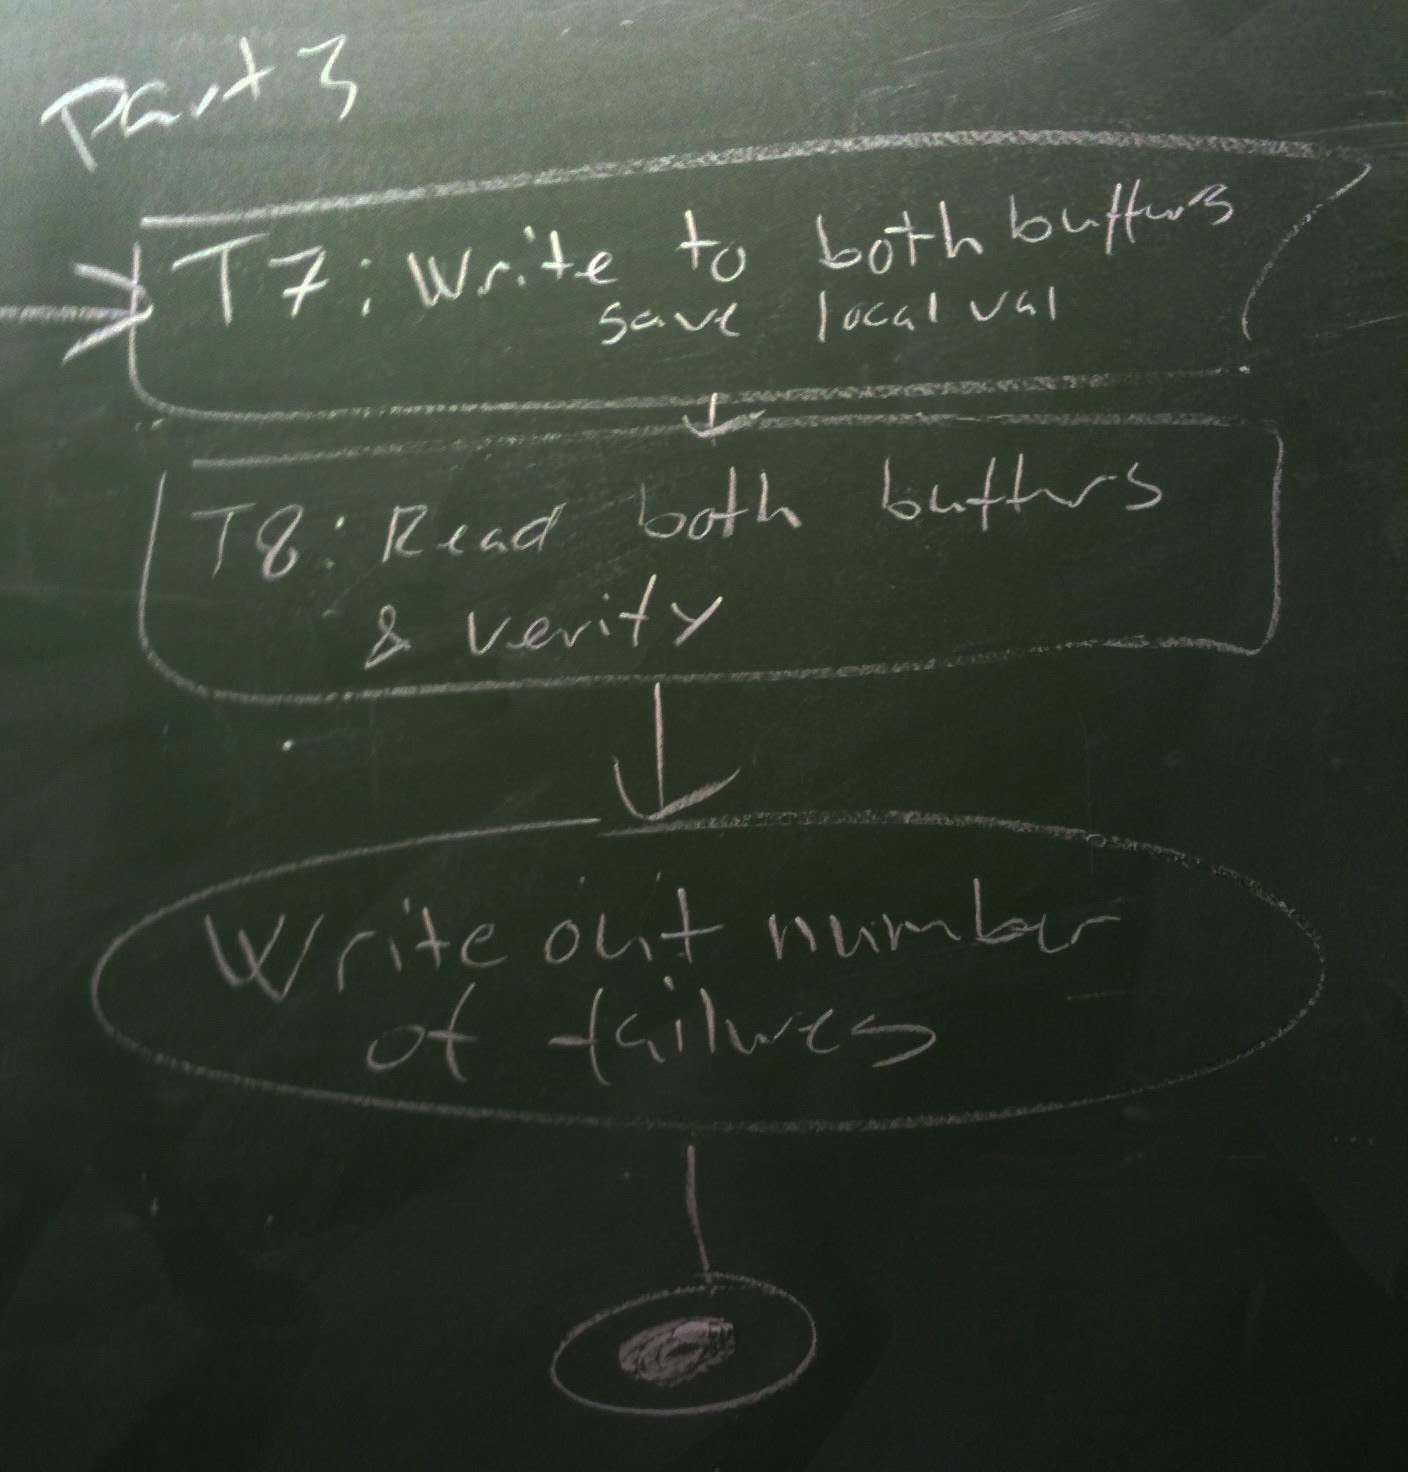
\includegraphics[width=0.6\textwidth]{part3.jpg}
		\caption{Part three of the test, writing/reading to two circular buffers}
	\end{centering}
\end{figure}
\newpage
\subsection{Function implementation}
The below picture shows an illustration of what functions are called when and with what parameters. Also a small drawing of a buffer has been created to illustrate that
the pointer should be 'returned' to the start of the array when it is increased, after having pointed at the last location in the array.
\begin{figure}[bh!]		%Remember to put the h!, to not fuck the sections.
	\begin{centering}
 		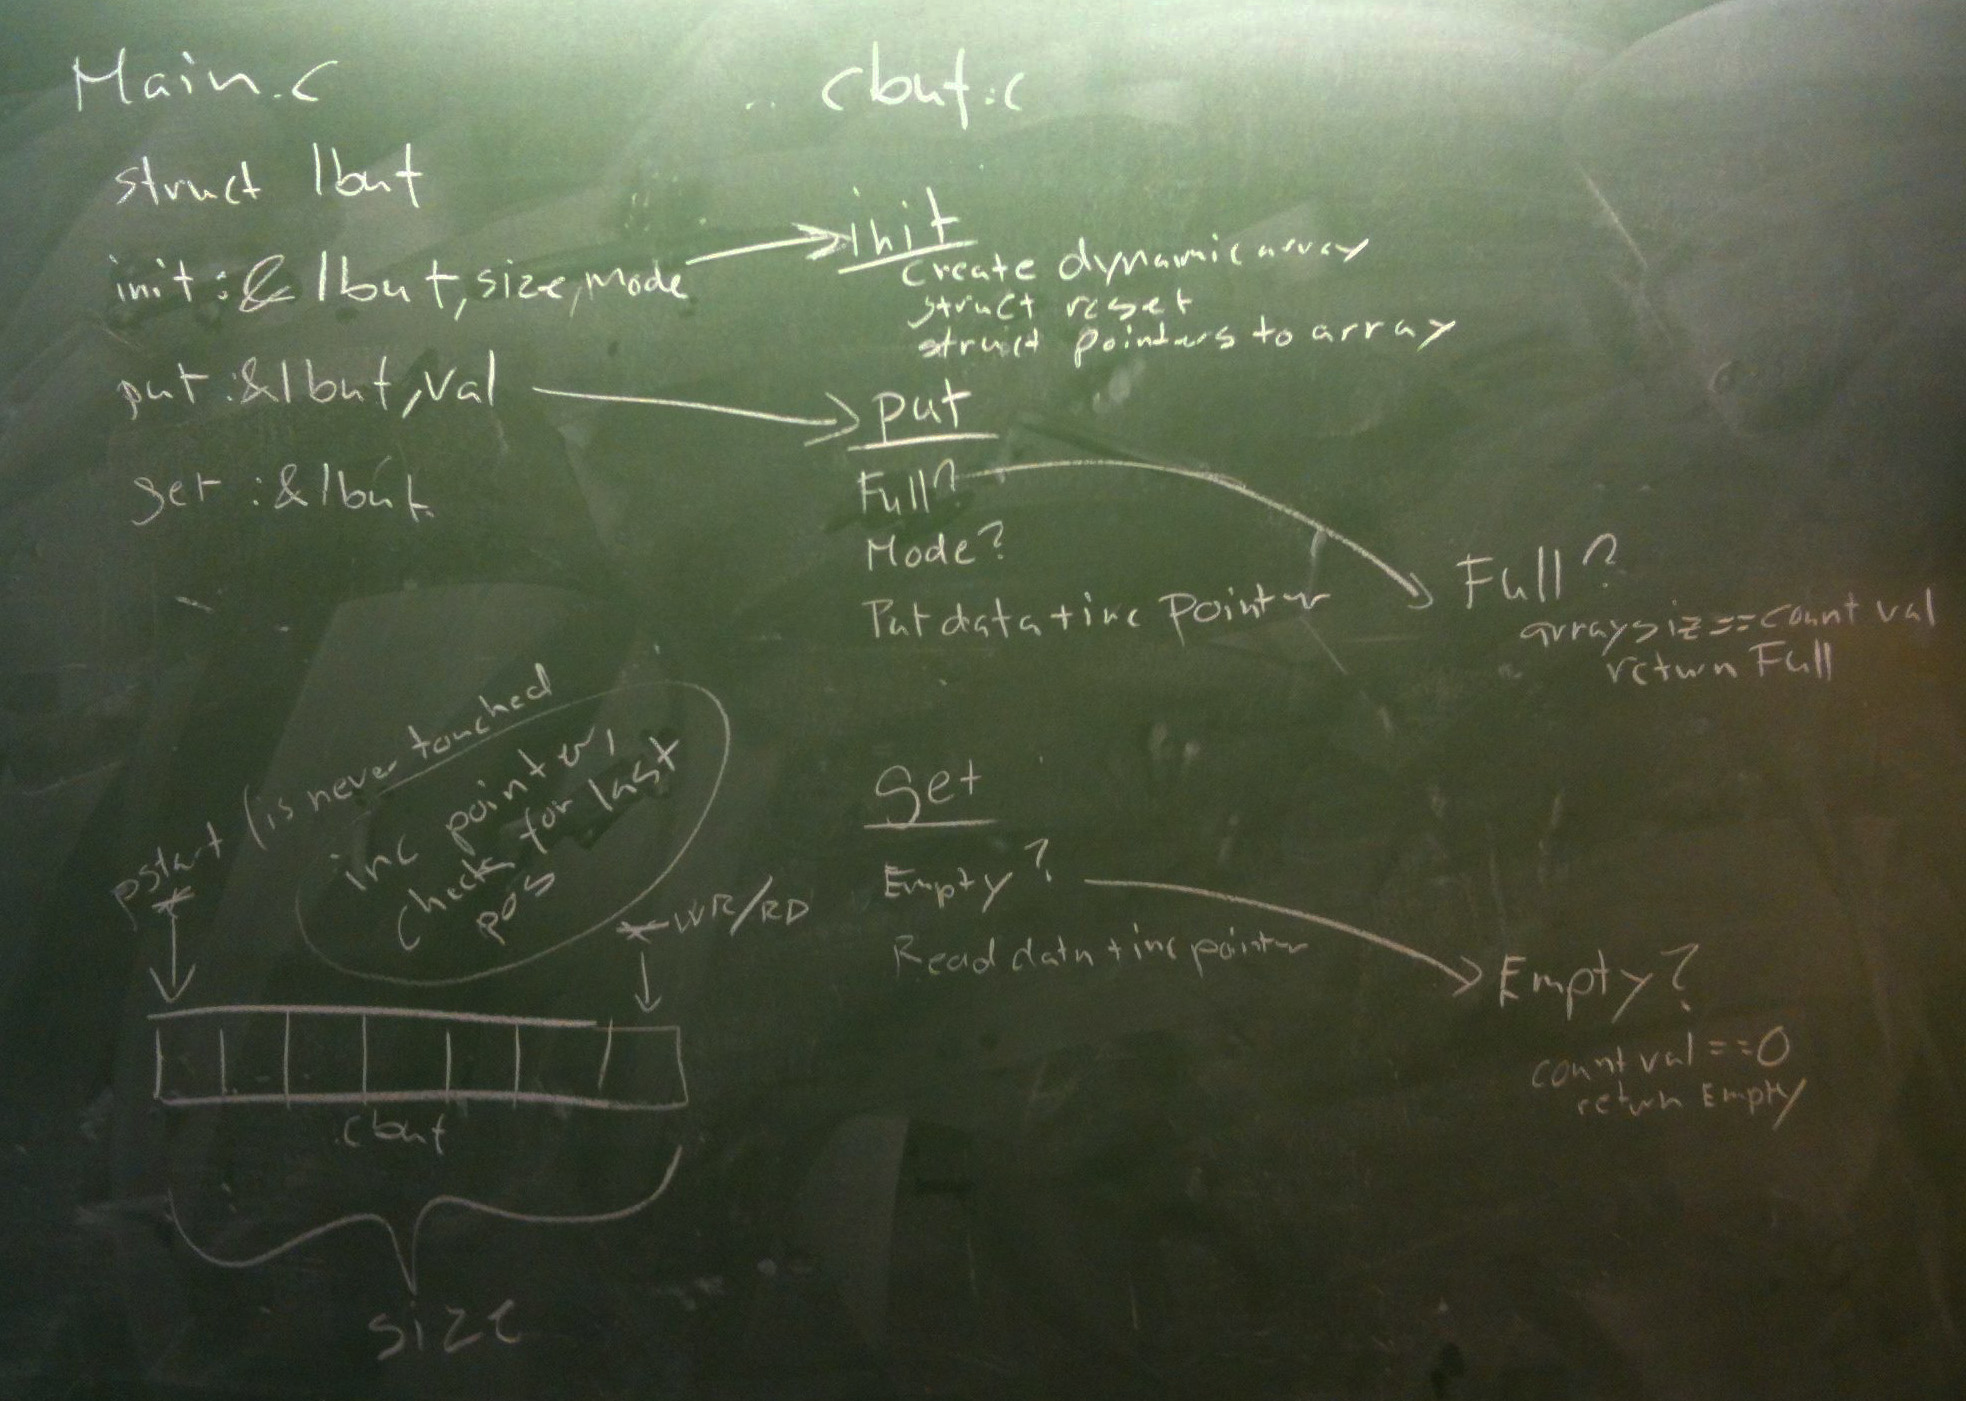
\includegraphics[width=1.0\textwidth]{files.jpg}
		\caption{Part three of the test, writing/reading to two circular buffers}
	\end{centering}
\end{figure}
\newpage
\section{Implementation (the code)}
\textbf{CircularBuffer.h}
\begin{lstlisting}
/*
 * CircularBuffer.h
 *
 *  Created on: Nov 15, 2011
 *      Author: Team3#Dennis
 */

#ifndef CIRCULARBUFFER_H_
#define CIRCULARBUFFER_H_

// Structures
typedef struct{
	int *p_rd;	//pointer to current read add of the buffer
	int *p_wr;	//pointer to current write add of the buffer
	int *p_start; //pointer to start of the buffer
	int count;	//continues the amount of data written to the buffer
	int mode;	//holds the mode of the buffer (overwrite / no overwrite)
	int size;	//size of the array
} cbuf, *pbuf;

// Prototypes
int put(cbuf *buf, int val);
int get(cbuf *buf);
int isEmpty(int count);
int isFull(int count, int size);
void initialise(cbuf *buf, int size, int overwrite);
void delete(cbuf *buf);

// Defines
#define FULL -1
#define EMPTY -2

#define NOOVERWRITE 0
#define OVERWRITE   1

#endif /* CIRCULARBUFFER_H_ */
\end{lstlisting}
\newpage
\textbf{The initialization function}
\begin{lstlisting}
/****************************************************************************
 * Description: void initialise(cbuf *buf, int size, int overwrite)
 *
 * The function creates an int array of a certain size (parameter decided)
 * All values and pointers in the cbuf structure are zeroed.
 *
 * Parameters:
 * 		*buf 		: Pointer to the circular buffer structure (type cbuf)
 *		size		: Defines the size of the array that is created
 * 		overwrite 	: bit indicating the mode of the buffer
 *
 ***************************************************************************/
void initialise(cbuf *buf, int size, int overwrite){
	int *array;		//create a pointer of type int
					//create an array[size] in the heap and make the pointer created point to it
	array=(int *) malloc(size*sizeof(int));

	buf->p_rd = array;		//Point p_rd pointer point to start of the array
	buf->p_wr = array;		//Point p_wr 	-11-
	buf->p_start = array;	//Point p_start -11-
	buf->count = 0;			//reset counter (keeps track of number of data in the buffer)
	buf->mode = overwrite;	//mode bit (overwrite on / off when buffer is full)
	buf->size = size;		//holds value of buffer size
}
\end{lstlisting}

\textbf{The put function}
\begin{lstlisting}
/****************************************************************************
 * Description: int put(cbuf *buf, int val)
 *
 * Checks if the buffer is full. If it is full and the mode is set to overwrite
 * Data is shiftet, so the read pointer still looks at the oldest value in the buffer.
 * If the overwrite is off, data is not written if the buffer is full.
 * If the buffer is not full, data is written and the write pointer is incremented.
 *
 * Parameters:
 * 		*buf 		: Pointer to the circular buffer structure (type cbuf)
 * 		val			: Value that should be written to the buffer
 *
 *		return		: -1 if buffer is full, 0 otherwise
 ***************************************************************************/
int put(cbuf *buf, int val){
	if(isFull(buf->count, buf->size) == FULL){	//Checks if buffer is full.
		if(buf->mode == NOOVERWRITE){			//Mode check
			return FULL;						//Return FULL flag if noowerwrite mode and buffer is full.
		}
		else if(buf->mode == OVERWRITE){		//Point read pointer to second oldest value if in overwrite mode
			if(buf->p_rd == buf->p_start+buf->size) buf->p_rd = buf->p_start;
			else buf->p_rd++;
		}
	}
	else{
		buf->count++;							//Increase count value (tells how much data the buffer contains)
	}

	*buf->p_wr = val;							//Put new data to the current position (write pointer)

		//If data has been written to the last place in the array, the pointer is pointed to the
		//start of the array. Otherwise the pointer is increased to point at the next data address.
	if(buf->p_wr == buf->p_start+buf->size) buf->p_wr = buf->p_start;
	else buf->p_wr++;

	return 0;
}
\end{lstlisting}
\textbf{The get function}
\begin{lstlisting}
/****************************************************************************
 * Description: int get(cbuf *buf)
 *
 * Checks if the buffer is empty, if it is not, then the oldest value is returned
 *
 * Parameters:
 * 		*buf 		: Pointer to the circular buffer structure (type cbuf)
 *
 *		return		: Oldest value in the buffer. -1 if buffer is empty
 ***************************************************************************/
int get(cbuf *buf){
	int val;

	if(isEmpty(buf->count) == EMPTY){	//Checks if buffer is empty
		return EMPTY;					//Return if there is no data to read -2
	}

	buf->count--;			//Decrease count value (tells how much data the buffer contains)

	val = *buf->p_rd;		//Read data from the current position (read pointer)

		//If data has been read from the last place in the array, the pointer is pointed to the
		//start of the array. Otherwise the pointer is increased to point at the next data address.
	if(buf->p_rd == buf->p_start+buf->size) buf->p_rd = buf->p_start;
	else buf->p_rd++;

	return val;				//Return read data from buffer. -1 if buffer is empty
}
\end{lstlisting}
\newpage
\textbf{The functions isEmpty}
\begin{lstlisting}
/****************************************************************************
 * Description: int isEmpty(int count)
 *
 * Checks if the buffer is empty
 *
 * Parameters:
 * 		count  	: number of data written to the buffer
 *
 *		return	: -2 if the buffer is empty, 0 otherwise
 ***************************************************************************/
int isEmpty(int count){
	if(count == 0){		//If count is 0, the array contains no data
		return EMPTY;	//EMPTY flag is returned
	}
	return 0;
}
\end{lstlisting}

\textbf{The functions isFull}
\begin{lstlisting}
/****************************************************************************
 * Description: int isFull(int count, int size)
 *
 * Checks if the buffer is full
 *
 * Parameters:
 *		size	: value containing the value of the cbuffer working on
 * 		count  	: number of data written to the buffer
 *
 *		return	: -1 if the buffer is full, 0 otherwise
 ***************************************************************************/
int isFull(int count, int size){
	if(count >= size){	//If the count value equal to the size of the array, the buffer is full
		return FULL;	//FULL flag is returned
	}
	return 0;
}
\end{lstlisting}

\newpage
\textbf{the test function (main.c)}
\begin{lstlisting}
#define SIZE 10

int main(void){
	int i, val, fail = 0;
	cbuf lbuf1, lbuf2;
	int array[SIZE*2];

	//Initialize a circular buffer with no overwrite mode.
	initialise(&lbuf1, SIZE, NOOVERWRITE);

	//Check 1: Buffer empty at start
	if(get(&lbuf1) != EMPTY) fail++;

	//Check 2: write until buffer is full, count number of data sent + save sent data in local array
	i=0;
	while(1){
		val = rand()%100;
		array[i] = val;
		if(put(&lbuf1, val) == FULL) break;
		i++;
		if(i>SIZE*2) break;		//Timeout
	}
	if(i != SIZE) fail++;

	//Check3: Read all data from buffer and compare to local array
	i=0;
	while(1){
		val = get(&lbuf1);
		if(val == EMPTY) break;
		if(val != array[i]) fail++;
		i++;
		if(i>SIZE*2) break;		//Timeout
	}
	if(i != SIZE) fail++;

	//Check4: Write + read data right after each other to avoid FULL flag, do this 3xSIZE of the array
	//		  In the end, check if the buffer is empty (as it should be).
	for(i=0; i<SIZE*3; i++){
		put(&lbuf1, i);
		val = get(&lbuf1);
		if(val == EMPTY) fail++;
		if(val != i) fail++;
	}
	if(get(&lbuf1) != EMPTY) fail++;

	//Initialize a circular buffer with overwrite mode on and a different size than the first buffer
	initialise(&lbuf2, SIZE*2, OVERWRITE);

	//Check5: Write twice size of data as the buffer is wide without getting any FULL flags
	for(i=0; i<SIZE*4; i++){
		if(put(&lbuf2, i) == FULL) fail++;
		if(i<SIZE*2) array[i] = i;
		else array[i-(SIZE*2)] = i;
	}

	//Check6: Check the overrun buffer for correct data
	i=0;
	while(1){
		val = get(&lbuf2);
		if(val == EMPTY) break;
		if(val != array[i]) fail++;
		i++;
		if(i>SIZE*4) break;		//Timeout
	}
	if(i != SIZE*2) fail++;

	//Check7: Write to both circular buffers (one with overwrite on, and one where it is off)
	i=0;
	while(1){
		val = rand()%100;
		if(put(&lbuf2, val*2) == FULL) break;
		if(put(&lbuf1, val) == FULL) break;
		array[i] = val;
		i++;
		if(i>SIZE*4) break;		//Timeout
	}
	if(i != SIZE) fail++;

	//Check8: Read both buffers and see if they contain the right data.
	i=0;
	while(1){
		val = get(&lbuf1);
		if(val == EMPTY) break;
		if(val != array[i]) fail++;
		val = get(&lbuf2);
		if(val == EMPTY) break;
		if(val != array[i]*2) fail++;
		i++;
		if(i>SIZE*2) break;		//Timeout
	}
	if(i != SIZE) fail++;

	// Write out number of errors, if any.
	if(fail > 0) printf("NUMBER OF FAILS: %d",fail);
	else printf("TEST OK");
	return 0;
}
\end{lstlisting}
\newpage
\begin{figure}[bh!]		%Remember to put the h!, to not fuck the sections.
	\begin{centering}
 		\includegraphics[width=0.8\textwidth]{GoToComic.png}
		\caption{DON'T GOTO in C}
	\end{centering}
\end{figure}
\end{document}
